\section{Predictive allocation tests and the reversal region}
\label{sec:predictivetests}

\subsection{Fixed protocol for heterogeneous recurrent pathways}

To distinguish prediction from a fitted response curve, we generate
a new fixed set of eight synthetic networks using seed 20261110.
Their pathway counts are \(2,4,6,8,2,4,6,8\), giving 40 pathways.
Each source and output population has two to four coordinates.
Dense off-diagonal entries have magnitude \(0.02\)--\(0.20\);
the diagonal leak exceeds each absolute row sum by an independent
margin in \(0.35\)--\(1.1\). Each internal matrix is then scaled
by a factor in \(0.5\)--\(1.6\). Alternating network cases have
positive or signed off-diagonal entries. Thus stability is fixed
by construction, and both populations contain recurrent cycles.
The forward matrix is positive and Frobenius-normalized.
Independent diagonal source and output drive intensities are in
\(0.35\)--\(1.7\). Cue and scalar readout vectors are uniform
unit vectors on their respective populations. These choices were
fixed before this run; networks are not selected for an allocation
effect or a ranking reversal.

At unit forward gain, 48-node Gauss--Legendre quadrature determines
the readout mean \(h_i\) and the separate local and propagated
variances \(L_i,S_i\) for windows \(T=0.35,1.6\). A stationary
source-drive calculation gives \(\kappa_i\). The derived
\(F_i=4h_i^2/S_i\) and \(C_{*,i}=\kappa_iL_i/S_i\) then predict
allocations without fitting a gain--discrimination curve.
Each network uses three budgets: \(0.25,1,4\) times its total
unit-gain excess cost \(\sum_i\kappa_i\). The same three budgets
are held fixed across the two windows, giving 48 settings.

For an independent numerical comparison, the optimization objective
uses the full generator at each candidate gain. A Lyapunov solve
computes its stationary covariance, and matrix-exponential integral
identities compute its cue mean and window variance. It does not
evaluate the rational cost law in the objective. Budget shares
\(z_i\) parameterize gains as
\(m_i=\sqrt{Bz_i/\kappa_i}\), with \(z_i\ge0\) and
\(\sum_i z_i=1\). The resulting full-state stationary cost is
also checked directly. Joint discrimination is optimized by SLSQP
from three fixed types of starts: uniform, seeded Dirichlet, and
the first-coordinate corner. All 144 joint starts converge; their
statuses and objectives are retained. Max--min discrimination is
checked by a separate epigraph optimization of the full-state
scores. The analytical unequal-ceiling max--min prediction uses
the scalar target equation derived in Sec.~\ref{sec:modularsupp}.

The maximum relative objective discrepancies are
\(2.5\times10^{-13}\) for joint and \(2.4\times10^{-11}\) for
max--min decoding. The largest joint budget-share discrepancy is
\(7.1\times10^{-7}\), and the largest relative total-cost error
is \(1.9\times10^{-14}\). Main Fig.~4(e,f) shows joint predictions
and gains over equal shares; Fig.~\ref{fig:strengthening}(c) gives
the independently optimized max--min comparison. These checks
validate the allocation predictions on full recurrent models;
they do not infer a biological distribution of optimal policies.

For joint utility \(U=d_{\rm joint}'^2\), the relative improvement
\(100(U^*-U_{\rm equal})/U_{\rm equal}\) ranges from
\(0.0067\%\) to \(44.6\%\), with median \(3.31\%\).
The medians at the two windows are \(7.40\%\) and \(2.95\%\).
The unit-gain matrices, drives, cues and all three budgets are
unchanged across windows. The median total variation of the
optimal joint shares between windows is \(0.101\), with total
variation defined as half the sum of absolute share changes
[Fig.~\ref{fig:strengthening}(d)]. Settings with nearly equal
prices and returns can have almost no benefit from reallocation;
the optimization does not imply that equal allocation is always
substantially inefficient.

\subsection{Fixed-cost region and explicit noise interventions}

Main Fig.~3(e) scans 141 rate ratios \(R\in[1.05,8]\) and
161 coupling ratios \(\gamma\in[1.01,8]\), giving 22,701
specified model points. Set \(a_s=R^{-1/2}\), \(a_f=R^{1/2}\),
so \(a_sa_f=1\). For each point choose
\[
 \kappa=[2a_sa_f(a_s+a_f)]^{-1},\qquad
 m_f^2=\frac{1.25712}{\kappa(1+\gamma^2)},\qquad m_s=\gamma m_f.
\]
Thus the entire grid has the same excess cost, not the same
absolute gains. The exact eventual-reversal interval is
\(\sqrt R<\gamma<R\). Requiring opposite rankings at both
\(T=0.5\) and \(T=3\) selects the narrower region
\[
 \frac{V_0(a_s,0.5)}{V_0(a_f,0.5)}<\gamma^2<
 \frac{V_0(a_s,3)}{V_0(a_f,3)}.
\]
All grid classifications agree with this interval; 3,057 grid
points pass the two-window test. The color encodes the smaller
of the two fractional winning margins, in percent. The largest
such minimum margin in this grid is \(11.1\%\). These counts
describe a chosen parameter grid, not a prevalence estimate or
a statistical significance calculation. A prescribed coarse subset
of 32 two-route settings, spanning four rate ratios, four coupling
ratios and two windows, is also checked by full-state Lyapunov
and matrix-exponential calculations rather than the scalar ratio.

The explicit noise interventions in main Fig.~3(c) hold the
couplings fixed. Removing local output drive ties the two
separations. Removing source drive changes their ratio but not
its crossing. These are mechanism controls, not matched-cost
comparisons between different drive covariances. Return-coupling,
colored-drive and temporal-weight sensitivity examples are preserved
in Fig.~\ref{fig:strengthening}(a), with their full grid and
unsuccessful cases reported in Sec.~\ref{sec:crosssupp}.

\subsection{A condition-violating control}

The local-noise endpoint test requires common signal and
propagated-noise terms and a common price coefficient. To expose
the consequence of violating these assumptions, multiply only
the slow route's source-drive intensity by four, keeping its
local output drive unchanged. Set the gains to \(1.17,0.90\),
so its excess-cost coefficient is four times larger and the
actual budget ratio remains \(6.76\) at total excess cost
\(1.25712\). The local-noise endpoint ratios remain four and
16. Nonetheless, no separation-rank crossing occurs on the tested
\(0.025\le T\le12\) range [Fig.~\ref{fig:strengthening}(b)].
Using the endpoint inequality without checking matching would
therefore be incorrect. This is not a failure of the individual
module law: the unequal \(F_i\) and \(C_{*,i}\) still give the
correct scores. The heterogeneous recurrent allocation tests
above deliberately allow unequal coefficients and do not assume
that their pathways satisfy the controlled reversal criterion.

\begin{figure}[!htbp]
\centering
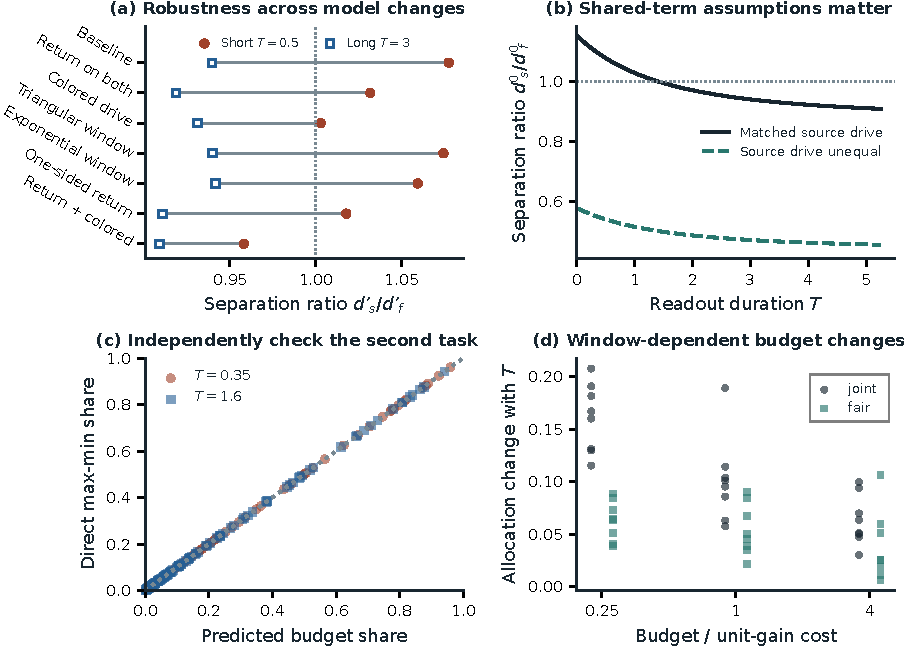
\includegraphics[width=\textwidth]{figures/fig_prrS_strengthening.pdf}
\caption{\textbf{Sensitivity, matching conditions and recurrent allocation.}
(a) Sensitivity examples with horizontal labels:
rust circles are \(T=0.5\), blue open squares \(T=3\). Return
coupling has magnitude \(0.05\), and colored-drive time constant
is \(0.5\); the combined case is retained. (b) Baseline matched
drive (dark solid) versus a fourfold source-drive mismatch on the
slow route (teal dashed), both at excess-cost ratio \(6.76\).
The latter does not satisfy the endpoint test's shared-term
assumptions. (c) Predicted versus full-state max--min budget shares
for the 48 heterogeneous recurrent settings. Colors and symbols
identify the two windows as in main Fig.~4(e); dotted line is
equality. (d) Total-variation changes in optimal budget shares
between \(T=0.35\) and \(1.6\), at each unchanged total budget.
Dark circles denote joint decoding and teal squares max--min;
each group contains eight fixed network examples. No biological
sampling or significance inference is intended.}
\label{fig:strengthening}
\end{figure}
